\documentclass[a4paper,twocolumn,11pt]{article}
\usepackage[utf8]{inputenc}
\usepackage[MeX]{polski}
\usepackage[top=3cm, bottom=3cm, left=2.5cm, right=2.5cm]{geometry}
\usepackage{subfigure}
\usepackage{amsfonts}
\usepackage{amsthm}
\usepackage{textcomp}
\usepackage{ragged2e}
\usepackage{tikz}
\usetikzlibrary{calc,shapes,shapes.multipart,arrows,chains}
\usepackage{tikz-uml}
\usepackage[explicit]{titlesec}
\usepackage{caption}

% ;;;;;;;;; macros ;;;;;;;;;;;;

\newlength{\mysize}
\newcommand{\mycfs}[1]{\setlength{\mysize}{#1pt}%
  \fontsize{\mysize}{1.2\mysize}\selectfont}
\newcommand{\mycfsb}[1]{\bfseries \mycfs{#1}}
\renewcommand{\captionfont}{\centering \mycfs{10}}
\renewcommand{\captionlabelfont}{\mycfsb{10}}

% ;;;;;;;;; headers ;;;;;;;;;;;;

\titleformat{\section}[runin]{\bfseries}{}{0pt}{\thesection. #1}[]
\titleformat{name=\section,numberless}[runin]{\bfseries}{}{0pt}{#1}[]
\titleformat{\subsection}[runin]{\bfseries}{}{0pt}{\thesubsection. #1}[]
\titlespacing*{\section} {0pt}{6pt}{2.3ex plus .2ex}
\titlespacing*{\subsection} {0pt}{3pt}{1.5ex plus .2ex}

% ;;;;;;;;; spacing ;;;;;;;;;;;;

\setlength\parindent{0.4cm}
\setlength{\columnsep}{0.8cm}

% ;;;;;;;;;;;;;;;;;;;;;;;;;;;;;;;;

\title{{\mycfsb{14} Aplikacja mobilna umożliwiająca umieszczenie wirtualnej grafiki w~rzeczywistym położeniu.}}
\author{{\mycfs{12} Michał Aniserowicz} \\ {\mycfs{11} Wydział Elektroniki i~Technik Informacyjnych} \\ {\mycfs{11} M.Aniserowicz@stud.elka.pw.edu.pl}}
\date{}

\begin{document}

\vspace{1.5cm}

\maketitle



%=========================================

\section*{Streszczenie}

\emph{
 Artkuł opisuje działanie przykładowej aplikacji mobilnej realizującej koncepcję rzeczywistości rozszerzonej.
 Zawiera także informacje na temat realizacji poszczególnych aspektów aplikacji.
 Najwięcej uwagi poświęcono wykorzystaniu sensorów wbudowanych w~urządzenia mobilne.
}



%=========================================

\section{Wstęp.}

Celem niniejszego artykułu jest wyjaśnienie działania i~ogólny opis poszczególnych aspektów aplikacji umożliwiającej umieszczenie wirtualnej grafiki w~rzeczywistym położeniu.

Rozdział \ref{sec:app_description} (``Opis aplikacji'') zawiera opis działania aplikacji i~wypunktowuje kolejne kroki pozyskiwania i przetwarzania wykorzystywanych przez nią danych.

Rozdział \ref{sec:position_tracking} (``Odczytywanie pozycji telefonu'') przybliża metody dokonywania odczytów położenia telefonu na kuli ziemskiej.
Wyjaśnia również znaczenie dokładności tych odczytów.

Rozdział \ref{sec:orientation_tracking} (``Odczytywanie orientacji telefonu'') przedstawia źródła informacji, na podstawie których telefon jest w~stanie określić swój obrót w układzie współrzędnych Ziemi.

Rozdział \ref{sec:image_rendering} (``Wyświetlanie obrazu'') opisuje biblioteki wykorzystywane przez system Android podczas renderowania obrazu. Zawiera także opis danych składających się na definicję wyświetlanego modelu i~informacje na temat jego obracania.

Rozdział \ref{sec:summary} podsumowuje artykuł.



%=========================================

\section{Opis aplikacji.} \label{sec:app_description}

Celem aplikaji opisywanej w niniejszym artykule jest umożliwienie użytkownikowi ``zastąpienia'' rzeczywistego obrazu obrazem wirtualnym, ``widzianym'' za pośrednictwem kamery telefonu klasy smartfon (aplikacja przeznaczona jest na platformę Android).
Taka funkcjonalność jest jedną z form realizacji koncepcji rzeczywistości rozszerzonej (ang. Augmented Reality)~\cite{aug:real}.

Działanie aplikacji zaczyna się od zdefiniowania pary obraz rzeczywisty-obraz wirtualny (zdefiniować można wiele takich par):

\begin{enumerate}
 \item Użytkownik wybiera obraz rzeczywisty (poprzez zrobienie jego zdjęcia), który będzie stanowił tło dla obrazu wirtualnego.
 \item Następuje odczyt współrzędnych geograficznych telefonu (patrz Rozdział~\ref{sec:position_tracking}).
 \item Następuje odczyt orientacji telefonu (patrz Rozdział~\ref{sec:orientation_tracking}).
 \item Użytkownik wybiera trójwymiarowy obiekt wirtualny, który ma zastąpić obraz rzeczywisty.
 \item Pozyskane dane zapisywane są w~bazie danych aplikacji.
\end{enumerate}

Następnie aplikacja cyklicznie próbuje rozpoznać którykolwiek ze zdefiniowanych obrazów rzeczywistych i~zastąpić go odpowiadającym mu obrazem wirtualnym:

\begin{enumerate}
 \item Wczytywany jest zbiór $R$~zdefiniowanych obrazów rzeczywistych.
 \item Następuje odczyt współrzędnych geograficznych telefonu.
 \item Ze zbioru $R$~usuwane są obrazy, podczas pozyskania których telefon znajdował się dalego od aktualnego położenia.
 \item Następuje odczyt orientacji telefonu.
 \item Ze zbioru $R$~usuwane są obrazy, podczas pozyskania których telefon był skierowany w~znacznie inną stronę niż aktualnie.
 \item Pobierany jest obraz $c$~z~kamery telefonu.
 \item Dla każdego obrazu $r$~z~$R$:
  \begin{itemize}
   \item $r$~jest obracany tak, aby zniwelować różnicę pomiędzy przypisaną do niego orientacją, a~orientacją aktualną (odczytaną w kroku 4),
   \item określany jest stopień podobieństwa $c$~do~$r$ (szczegóły tej operacji wykraczają poza tematykę niniejszego artykułu).
  \end{itemize}
 \item Z $R$~usuwane są obrazy o~nieakceptowalnie małym stopniu podobieństwa do $c$.
 \item Z $R$~wybierany jest obraz $r_f$~o~największym stopniu podobieństwa do $c$.
 \item Na ekranie telefonu wyświetlany jest obraz $c$~z~nałożonym na niego (odpowiednio obróconym) obrazem $r_f$.
\end{enumerate}

Jeśli w~którymkolwiek kroku zbiór $R$~stanie się pusty, algorytm kończy działanie, a~na ekranie telefonu wyświetlany jest obraz pobrany z~kamery urządzenia.



%=========================================

\section{Odczytywanie pozycji telefonu.} \label{sec:position_tracking}

System Android udostępnia możliwość odczytywania pozycji telefonu na kuli ziemskiej z~następujących źródeł~\cite{and:loc}:

\begin{itemize}
 \item odbiornik GPS,
 \item metoda Assisted GPS,
 \item odczyt pasywny.
\end{itemize}


\subsection{Odbiornik GPS.}
 Pierwsza z metod polega na odczycie bezpośrednio z~odbiornika GPS zamontowanego w~urządzeniu.
 Jest to najdokładniejszy sposób określania pozycji telefonu - jego dokładność wynosi od kilku do kilkunastu metrów.
 Ma jednak znaczące ograniczenia:
 \begin{itemize}
  \item ze względu na konstrukcję systemu GPS, do poprawnego działania wymaga otwartej przestrzeni - używanie go w~budynkach lub w~ich pobliżu skutkuje niedokładnymi odczytami,
  \item przed uzyskaniem pierwszego odczytu musi nawiązać kontakt z~kilkoma (ok. 7) satelitami GPS, co może potrwać nawet do kilku minut,
  \item pobiera najwięcej energii spośród wszystkich źródeł.
 \end{itemize}


\subsection{Assisted GPS.}
 Metoda Assisted GPS (AGPS, wspomagany GPS) oprócz odbiornika GPS wykorzystuje sygnał sieci komórkowej.
 Telefon otrzymuje od pobliskich stacji bazowych informacje na temat dostępności satelitów GPS oraz przybliżonych pozycji tych satelitów.
 Znacząco przyśpiesza to uzyskanie pierwszego odczytu, a~także eliminuje wymóg otwartej przestrzeni.
 Co więcej, AGPS pobiera mniej energii niż bezpośredni odczyt GPS.
 Jego wadą jest jednak dokładność - posiłkowanie się przybliżonymi danymi pochodzącymi ze stacji bazowych powoduje jej spadek do kilkudziesięciu metrów.


\subsection{Odczyt pasywny.}
 Metoda odczytu pasywnego nie korzysta z odbiornika GPS - jest więc najmniej dokładna (jej dokładność wynosi od kilkudziesięciu do kilkuset metrów).
 Polega na porównaniu siły sygnału odbieranego przez urządzenie od pobliskich stacji bazowych.
 Znając lokalizajcję stacji bazowych, możliwe jest przybliżone określenie pozycji urządzenia.
 Dodatkowym źródłem informacji jest siła sygnału pochodzącego od sieci Wi-Fi wykrywanych przez urządzenie\footnote{Firma Google, podobnie jak inne firmy działające w~sektorze mobilnym, zbiera i~przechowuje informacje o~lokalizacji sieci bezprzewodowych~\cite{wifi:loc}.}.\\

Wyboru źródła odczytu dokonuje programista, poprzez jawne wskazanie, którego dostawcy lokalizacji (ang. \emph{LocationProvider}) chce użyć.
Może również zdać się na system, formułując jedynie kryteria wyboru, takie jak wymagana dokładność odczytu, możliwość uzyskania informacji o~prędkości poruszania się urządzenia i~kierunku jego ruchu, czy zezwolenie na użycie metody, która wiąże się z~naliczeniem opłat przez operatora sieci.


\subsection{Problem niedokładności odczytów.}
 Używając nawet najdokładniejszej z metod, błąd odczytu odbiornika GPS waha się od kilku do kilkunastu metrów, w~zależności od miejsca odczytu.
 O ile błąd na poziomie dwóch-trzech metrów w wielu przypadkach można uznać za akceptowalny, o~tyle niedokładność rzędu dwunastu-piętnastu metrów może bardzo niekorzystanie wpływać na doświadczenia użytkowników aplikacji intensywnie korzystających z~informacji o~położeniu telefonu na kuli ziemskiej.
 
 Za przykład posłużyć może gra w~``policjantów i~złodziei'', w~której osoba goniąca przez cały czas jest informowana o~tym, jaki dystans powinna przebyć i~w jakim kierunku się poruszać, aby dotrzeć do osoby uciekającej.
 Dystans ten typowo wynosił będzie od zera do kilkuset metrów.
 
 Załóżmy, że w~danym momencie policjant znajduje się w~okolicach wydziału Elektroniki i~Technik Informacyjnych (punkt A(52,219505\textdegree~N, 21,012028\textdegree~E)), a~złodziej - na ulicy Lwowskiej (w punkcie B(52,220458\textdegree~N, 21,012281\textdegree~E)).
 Odległość między punktami wynosi 103~m, a~azymut - 9,24\textdegree.
 Następują odczyty pozycji policjanta i~złodzieja, oba z~niedokładnością około dziesięciu metrów.
 Według odczytów, policjant znajduje się w~punkcie A'(52,219518\textdegree~N, 21,011892\textdegree~E), a~złodziej w~punkcie B'(52,220466\textdegree~N, 21,012431\textdegree~E).
 
 Obliczenia dla tych punktów wskazują, że policjant powinien przebyć 115,3~m w~kierunku 19,2\textdegree.
 Niedokładność wskazań jest na tyle duża, że może zmylić policjanta - zamiast na ulicę Lwowską, prawdopodobnie pobiegnie on w~kierunku ulicy Śniadeckich (sytuację obrazuje Rysunek~\ref{fig:positionTracking}).

\begin{figure}[!ht]
 \begin{center}
  \scalebox{0.55}
  {
   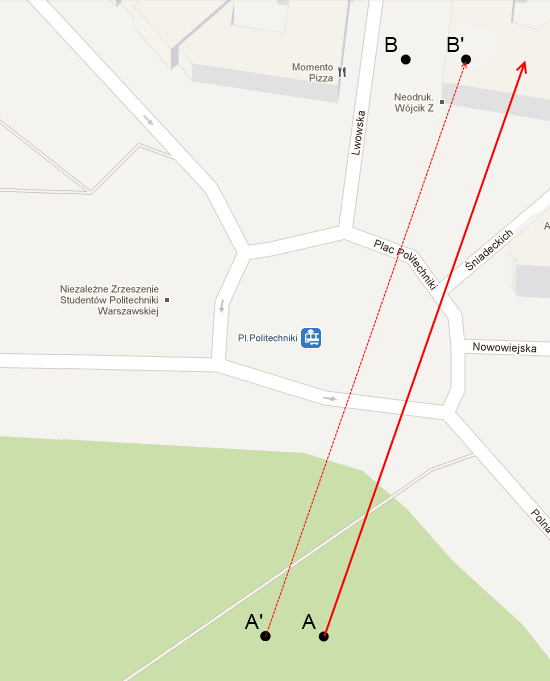
\includegraphics{figures/positionTracking.png}
  }
 \end{center}
 \caption{
  Pesymistyczny przykład konsekwencji błędu odczytu pozycji.
  Linią przerywaną zaznaczono wynik dokonanego odczytu, a linią ciagłą - to, jak wynik zostanie zinterpretowany przez użytkownika.
  [Źródło mapy: https://maps.google.pl/]
 }
 \label{fig:positionTracking}
\end{figure}

 
 Jak widać, dokładność jest istotna nawet w~sytuacjach, w~których odległość pomiędzy telefonami wynosi ponad sto metrów.
 W przypadku metod odczytu udostępnianych przez system Android, nie jest możliwe całkowite usunięcie błędu odczytu - wynika on z jakości odbiorników GPS montowanych w smartfonach. Można jednakże próbować go zmniejszyć poprzez rozszerzenie istniejących metod o~operacje korygujące, takie jak filtrowanie lub uśrednianie kolejnych odczytów.



%=========================================

\section{Odczytywanie orientacji telefonu.} \label{sec:orientation_tracking}

Źródłem wiedzy o~obrocie własnym urządzenia są odczyty z~wbudowanych w~telefon sensorów: akcelerometru, magnetometru i~żyroskopu.


\subsection{Akcelerometr.}
 Akcelerometr dostarcza informacji o~przyśpieszeniach działających na telefon.
 Przykładowo, jeśli telefon trzymany jest pionowo w miejscu, to działa na niego jedynie siła grawitacji, dając odczyt wynoszący około $9,81\frac{m}{s^2}$ na osi $y$.
 Zorientowanie osi obrazuje Rysunek \ref{fig:accelerometer_axes}.
 
 \begin{figure}[!ht]
 \begin{center}
  \scalebox{0.6}
  {
   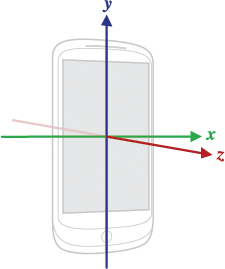
\includegraphics{figures/accelerometer_axes.png}
  }
 \end{center}
 \caption{Zorientowanie osi telefonu dla odczytów akcelerometru~\cite{and:doc:phone:axes}.}
 \label{fig:accelerometer_axes}
\end{figure}


 Na podstawie informacji o tym, na jakie osie i~w~jakim stopniu działa siła grawitacji, można wnioskować o~nachyleniu telefonu.
 Jako że akcelerometr mierzy przyśpieszenie wypadkowe, podczas ruchu urządzenia wnioskowanie to jest obarczone dużym błędem.
 Aby zminimalizować błąd, w~systemie Android zastosowano filtr dolnoprzepustowy, który częściowo odcina wpływ poruszania na dokładność odczytów.


\subsection{Magnetometr.}
 Magnetometr odczytuje wartości pola magnetycznego otaczającego urządzenie.
 Na podstawie tych wartości można określić, w~którą stronę świata zwrócony jest telefon.
 Sensor podaje odczyty dla wszystkich trzech osi - orientacja urządzenia nie jest więc przeszkodą.
 Należy jednak zwrócić uwagę na to, że odczyty nie mają szansy być bardzo dokładne - magnetometr mierzy nie tylko pole magnetyczne Ziemi, ale także pola generowane przez inne podzespoły telefonu, na przykład głośnika.\\


Połączone dane z~akcelerometru i~magnetometru pozwalają określić przybliżoną orientajcę telefonu.


\subsection{Żyroskop.}
 Dokładniejszy wynik można jednak otrzymać korzystając z~żyroskopu, montowanego głównie w~telefonach z~wyższej półki.
 Mierzy on prędkość kątową telefonu wokół każdej z osi.
 Na podstawie prędkości kątowej możliwe jest wyznaczenie wartości kąta obrotu, czyli uzyskanie informacji o~orientacji urządzenia.



%=========================================

\section{Wyświetlanie obrazu.} \label{sec:image_rendering}

Do generowania grafiki trójwymiarowej system Android wykorzystuje biblioteki OpenGL ES (OpenGL for Embedded Systems).
Jest to odmiana biblioteki OpenGL dedykowana dla systemów wbudowanych używanych między innymi w~konsolach i~telefonach~\cite{ogl:es}.
Android oferuje wsparcie dla dwóch standardów biblioteki:

\begin{itemize}
 \item OpenGL ES 1.x - wykorzystuje potok ustalony (ang. fixed pipeline).
  Oznacza to, że transformacje oraz obliczenia koloru wierzchołków wykonywane w~celu imitacji cieniowania i~oświetlenia wykonywane są przez kartę graficzną w~sposób narzucony z~góry.
  Utrudnia to lub uniemożliwia uzyskanie wielu zaawansowanych efektów graficznych, takich jak mapowanie wypukłości\footnote{Mapowanie wypukłości (ang. bump mapping) - technika umożliwiająca symulowanie obiektów o~porowatej powierzchni.}, płaszczyzny refleksji\footnote{Płaszczyzny refleksji (ang. reflection planes) - technika umożliwiająca uzyskanie efektu lustrzanego odbicia sceny na danej powierzchni.}~\cite{tec:3d} czy renderowanie z~użyciem szerokiego zakresu dynamicznego\footnote{Renderowanie z~użyciem szerokiego zakresu dynamicznego (ang. high dynamic range rendering) - technika umożliwiająca uzyskanie realistycznego oświetlenia przez wierne odwzorowanie bardzo jasnych i~ciemnych elementów sceny.}~\cite{nvi:hdr}. 
 \item OpenGL ES 2.x - wykorzystuje potok programowalny (ang. programmable pipeline).
  Umożliwia pisanie krótkich programów w~języku GLSL\footnote{GLSL - OpenGL Shading Language, http://www.\\opengl.org/documentation/glsl/.} nazywanych shaderami, które definiują sposób wykonywania obliczeń na wierzchołkach.
  Umożliwia to uzyskiwanie zaawansowanych efektów graficznych. Jest jednak trudne do zrozumienia dla początkujących programistów, gdyż wykonywanie transformacji lub oświetlenie sceny wymaga podania kodu źródłowego tych operacji jako wartości zmiennych napisowych (\emph{String}) - poprawność tego kodu nie jest sprawdzana przez kompilator, co znacznie utrudnia wykrycie ewentualnego błędu.
\end{itemize}


\subsection{Definicja modelu.}
 Renderowany na ekranie model opisany jest trójkątnymi ścianami.
 Do jego zdefiniowania wymagane są następujące informacje:

 \begin{itemize}
  \item tablica współrzędnych wierzchołków obiektu - każdy wierzchołek opisany jest trzema współrzędnymi $(x, y, z)$,
  \item tablica kolorów wierzchołków obiektu - każdy wierzchołek opisany jest czterema wartościami $(r, g, b, a)$ definiującymi jasności kanałów: czerwonego, zielonego, niebieskiego i~przezroczystości.
 \end{itemize}


\subsection{Obracanie modelu.}
 Aby utrzymać model w~pozycji pozornie nieruchomej względem otoczenia telefonu, niezbędna jest wiedza o~aktualnej orientacji urządzenia i~obracanie modelu przeciwnie do tej orientacji.
 
 Klasa \emph{SensorManager} należąca do API systemu Android udostępnia operację (\emph{getRotationMatrix}) pozwalającą wyznaczyć macierz obrotów telefonu.
 Macierz tę można zastosować do konwersji współrzędnych punktu z~układu współrzędnych telefonu do układu współrzędnych jego otoczenia (zorientowanie osi otoczenia przedstawia Rysunek \ref{fig:orientation_axes}).
 Aby ją uzyskać, należy pobrać odczyty akcelerometru i~magnetometru (lub żyroskopu) i~przekazać je metodzie \emph{getRotationMatrix}.

 \begin{figure}[!ht]
 \begin{center}
  \scalebox{0.6}
  {
   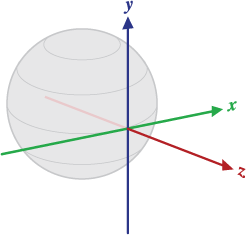
\includegraphics{figures/orientation_axes.png}
  }
 \end{center}
 \caption{Zorientowanie osi świata dla orientacji telefonu~\cite{and:doc:world:axes}.}
 \label{fig:orientation_axes}
\end{figure}



\subsection{Orientacja urządzenia a tryb wyświetlania.}
 Macierz obrotu zwracana przez metodę \emph{getRotationMatrix} przechowuje wartości określające fizyczną orientację telefonu.
 Obrót modelu według tych wartości będzie niepoprawny, jeśli ekran urządzenia będzie wyświetlał treści w~trybie innym niż domyślny.
 Dwa podstawowe tryby wyświetlania, to:
 \begin{itemize}
  \item portrait mode (tryb portretu, domyślny) - tryb używany, gdy telefon znajduje się pozycji pionowej,
  \item landscape mode (tryb krajobrazu) - tryb używany w pozycji poziomej; interfejs graficzny aplikacji jest odpowiednio obrócony.
 \end{itemize}
 
 Przełączanie pomiędzy trybami odbywa się automatycznie w zależności od pozycji, w~jakiej znajduje się urządzenie.
 Zachowanie to można wyłączyć korzystając z~ustawień systemu, a~także kontrolować z~poziomu aplikacji - dlatego wyznaczenie poprawnej macierzy obrotów jedynie na podstawie odczytów sensorów nie zawsze jest możliwe.
 
 Android udostępnia informacje o aktualnie stosowanym trybie wyświetlania (dostarcza ich metoda \emph{getRotation} klasy \emph{Display}).
 W~przypadku, gdy jest on inny od domyślnego, macierz należy skorygować, tzn. zamienić miejscami dwie z~trzech osi.
 Na przykład przy obrocie ekranu o 90\textdegree~w~prawo, oś $y$ wskazuje tam, gdzie poprzednio wskazywała oś $x$, a~oś $x$ - w kierunku przeciwnym do pierwotnie wskazywanego przez oś $y$.
 Podając macierz obrotu i~sposób zamiany osi jako argumenty operacji \emph{remapCoordinateSystem} klasy \emph{SensorManager}, uzyskać można skorygowaną macierz.

 Skorygowana macierz obrotu bez dalszych modyfikacji może zostać użyta do obrócenia wyświetlanego modelu tak, aby zniwelować obrót urządzenia.
 Rysunek \ref{fig:spaceGraphics_orientation} prezentuje kilka przykładów wyświetlania obróconego modelu.
 
 \begin{figure}[!ht]
 \begin{center}
  \subfigure[]{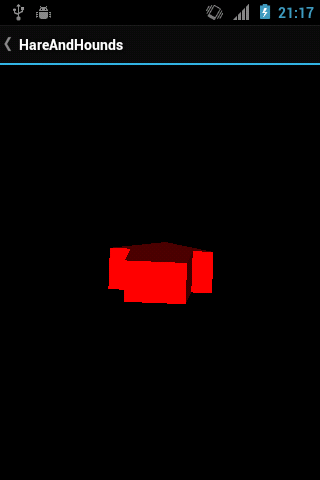
\includegraphics[width=0.2\textwidth]{figures/spaceGraphics_orientation_VerN.png}}
  \subfigure[]{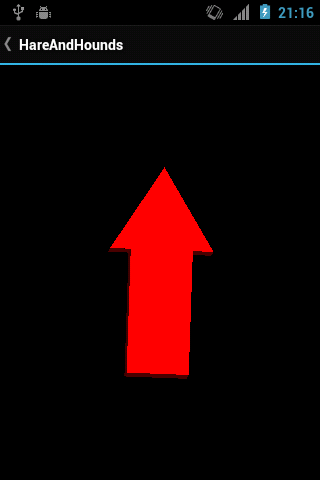
\includegraphics[width=0.2\textwidth]{figures/spaceGraphics_orientation_HorN.png}}\\
  \subfigure[]{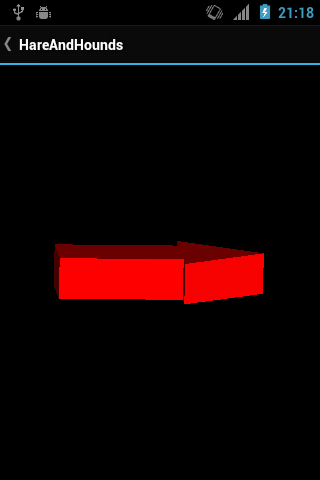
\includegraphics[width=0.2\textwidth]{figures/spaceGraphics_orientation_VerW.png}}
  \subfigure[]{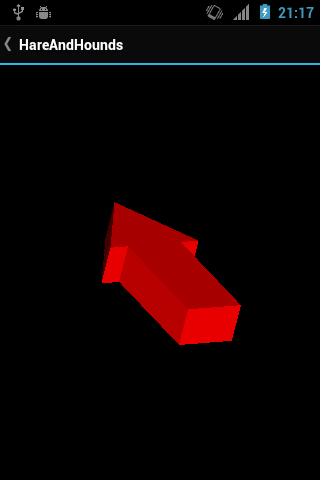
\includegraphics[width=0.2\textwidth]{figures/spaceGraphics_orientation_mixed.png}}
 \end{center}
 \caption{
  Przykłady obróconego modelu strzałki wsazującej północ:
  (a) telefon trzymany pionowo, skierowany na północ;
  (b) telefon leżący poziomo, skierowany na północ;
  (c) telefon trzymany pionowo, skierowany na zachód;
  (d) telefon skierowany lekko w dół i~na prawo od północy.
 }
 \label{fig:spaceGraphics_orientation}
\end{figure}




%=========================================

\section{Podsumowanie.} \label{sec:summary}

Realizacja koncepcji rzeczywistości rozszerzonej w~aplikacjach mobilnych wymaga wykorzystania wielu sensorów zamontowanych w telefonach (GPS, żyroskop, akcelerometr, magnetometr, kamera).
Główne problemy tego typu aplikacji to niedokładność odczytów sensorów i ich zapotrzebowanie na energię, a także potrzeba wyświetlania grafiki tak, aby zapewnić użytkownikowi jak najbardziej realistyczne doznania.

%=========================================

\begin{thebibliography}{9}
 \small

 \bibitem{aug:real} \emph{Rzeczywistość rozszerzona.}
                              Wikipedia.
                              dostęp: maj 2014.
                              w: http://pl.wikipedia.org/wiki/\\Rzeczywisto\%C5\%9B\%C4\%87\_rozszerzona

 \bibitem{and:loc} Cejas, Fernando.
                   (28.10.2010).
                   \emph{Android Location Providers - gps, network, passive.}
                   dostęp: maj 2014.
                   w: http://www.android10.org/\\index.php/articleslocationmaps/226-android-location-providers-gps-network-passive/
 
 \bibitem{wifi:loc} Vaughan-Nichol, Steven J.
                    \emph{How Google--and everyone else--gets Wi-Fi location data.}
                    dostęp: maj 2014.
                    w: http://www.zdnet.com/\\blog/networking/how-google-and-everyone-else-gets-wi-fi-location-data/1664/

 \bibitem{and:doc:phone:axes} \emph{SensorEvent.}
                              Android Developers.
                              dostęp: maj 2014.
                              w: http://developer.android.com/\\reference/android/hardware/SensorEvent.html

 \bibitem{and:doc:world:axes} \emph{SensorManager.}
                              Android Developers.
                              dostęp: maj 2014.
                              w: http://developer.android.com/\\reference/android/hardware/SensorManager\\.html\#getRotationMatrix(float[], float[], floa\\t[], float[])

 \bibitem{ogl:es} \emph{OpenGL ES - The Standard for Embedded Accelerated 3D Graphics.}
                  dostęp: maj 2014.
                  w: http://www.khronos.org/opengles/

 \bibitem{tec:3d} \emph{Advanced Shaders.}
                  dostęp: maj 2014.
                  w: http://www.techsoft3d.com/getting-started/\\hoops-visualize/advanced-shaders

 \bibitem{nvi:hdr} Green S., Cebenoyan C.
                   \emph{High Dynamic Range Rendering on the GeForce 6800.}
                   dostęp: maj 2014.
                   w: http://download.nvidia.com/\\developer/presentations/2004/6800\_Leagues/\\6800\_Leagues\_HDR.pdf

\end{thebibliography}

\end{document}
